\documentclass[a4paper]{article}
\usepackage{amsmath}
\usepackage{amssymb}
\usepackage{amsthm}
\usepackage{hyperref}
\usepackage{graphicx}

\theoremstyle{definition}
\newtheorem{example}{Example}[subsection]
\newtheorem{lemma}{Lemma}[subsection]

\begin{document}

\title{A Primer on Optimization}
\author{Saniya Maheshwari \\ \texttt{saniya@firstcry.in}}
\date{\today}
\maketitle

\begin{abstract}
	This article is a short introduction to the subject of optimization.
	The only mathematical background assumed is a basic understanding of linear algebra and multivariable calculus, and the language has been kept as straightforward and lucid as possible so that it is easy to follow along.

	We present the basic theory of optimization problems, including the important subclass of convex problems, as well as Lagrange multipliers, the duality framework, and the KKT conditions.
	In order to give a flavour of how optimization problems are formulated and interpreted, we also present some simple applications, including % TODO
	Finally, to develop an understanding for how such problems are solved in practice, we also present some of the popular iterative algorithms, including % TODO

	After reading this article, we hope that the reader will be able to better appreciate and understand optimization problems arising in a variety of fields.
\end{abstract}

\section{Introduction}

\subsection{Notation}

In this article, we are going to work with a lot of vectors and matrices.
Generally, we will denote matrices with capital letters, for e.g. $A$.
As far as vectors are concerned, we won't use any specific notation to distinguish them from scalars, i.e. we won't use notation such as $\bar{a}$ or $\vec{a}$.
Instead, notation such as the following will make it clear whether a quantity is a scalar or a vector: $a \in \mathbb{R}$ implies that $a$ is a (real-valued) scalar, and $a \in \mathbb{R}^n$ implies that $a$ is a (real-valued) $n$-dimensional vector.
We will also use a similar notation for matrices, i.e. $A \in \mathbb{R}^{m \times n}$ implies that $A$ is a (real-valued) matrix of order $m$ by $n$.

We will use subscript notation to denote the elements of a vector or matrix.
In other words, $a_i$ denotes the element at position $i$ of a vector $a$, and $A_{ij}$ denotes the element at position $(i, j)$ of a matrix $A$.

Another notation that we will frequently use pertains to component-wise inequality between two vectors.
The standard convention is to use the signs $\prec$, $\succ$, $\preceq$, and $\succeq$ in place of the usual signs $<$, $>$, $\leq$, and $\geq$ respectively.
For example, given two $n$-dimensional vectors $a$ and $b$, the expression $a \preceq b$ implies that $a_i \leq b_i$ for all $i$ from 1 to $n$.
For equality and ``non-equality" we use the signs $=$ and $\neq$ as usual.

These comparison signs will also be used to compare vectors and scalars (component-wise, of course).
For example, given an $n$-dimensional vector $a$, the expression $a = 0$ implies that $a_i = 0$ for all $i$ from 1 to $n$.

Finally, we will also use notation of the kind $f : A \rightarrow B$, which you must be familiar with if you know the basics of functions.
This notation depicts that we have a function $f$ with domain $A$ and range $B$, i.e. its input always lies in the set $A$ and its output always lies in the set $B$.
The most common way in which we use this notation is $f : \mathbb{R}^n \rightarrow \mathbb{R}$, which illustrates that the function $f$ takes a (real-valued) $n$-dimensional vector as input and produces a (real-valued) scalar as output.

Other notations and conventions will be introduced as required in this article.

\subsection{Hyperplanes}

The concept of a \textit{hyperplane} will come up multiple times in this article.
Loosely speaking, a hyperplane is the $n$-dimensional generalization of a line and a plane.
Just as in two-dimensional space, we have a one-dimensional line, and in three-dimensional space we have a two-dimensional plane, similarly in any $n$-dimensional space, an $(n{-}1)$-dimensional \textit{subspace} of that space is called a hyperplane.

More formally, the hyperplane in $n$-dimensional space is defined as the set of all $x \in \mathbb{R}^n$ that satisfy
\begin{equation*}
	a^T x + b = 0
\end{equation*}
where $a \in \mathbb{R}^n$, $a \neq 0$, and $b \in \mathbb{R}$.
You can see how this is a generalization of the equations of a line and a plane: if you plug in $n = 2$, then this becomes
\begin{align*}
	\begin{bmatrix}
		a_1 & a_2
	\end{bmatrix}^T
	\begin{bmatrix}
		x_1 & x_2
	\end{bmatrix} + b & = 0 \\
	\Rightarrow a_1 x_1 + a_2 x_2 + b & = 0
\end{align*}
which is a line.
Similarly plugging in $n = 3$ will give us a plane.

\subsection{Norms}
\label{norms}

When it comes to vectors and matrices, an important quantity is the \textit{norm}.
The vector norm, commonly denoted with double bars such as these $\| \cdot \|$, is a function that yields some measure of the ``size" of the given vector.
For example, the most common vector norm is the Euclidean or $l_2$-norm, denoted as $\| \cdot \|_2$, which is defined as the square root of the sum of the squares of the elements of the given vector, i.e. if $a \in \mathbb{R}^n$, we have
\begin{equation*}
	\| a \|_2 = \sqrt{a_1^2 + a_2^2 + \dots + a_n^2}
\end{equation*}
Another popular norm is the $l_1$-norm, denoted as $\| \cdot \|_1$, which is defined as the sum of the absolute values of the elements of the vector.
\begin{equation*}
	\| a \|_1 = | a_1 | + | a_2 | + \dots + | a_n |
\end{equation*}

There are many other vector norms.
All of them typically follow three properties:
\begin{enumerate}
	\item Nonnegativity: for all vectors $a \in \mathbb{R}^n$, we must have $\| a \| \geq 0$, and $\| a \| = 0$ if and only if $a = 0$.
	\item Positive homogeneity: for all vectors $a \in \mathbb{R}^n$, given any positive scalar $c$, i.e. $c \in \mathbb{R}$ and $c > 0$, we must have $\| ca \| = c \| a \|$.
	\item Triangle inequality: the inequality $\| a + b \| \leq \| a \| + \| b \|$ must hold for all vectors $a, b \in \mathbb{R}^n$.
\end{enumerate}
The $l_1$- and $l_2$-norms follow these properties as well.\footnote{
You can readily verify that the first two properties indeed hold for both norms.
The third property holds for the $l_1$-norm by virtue of the fact that the absolute value function obeys the triangle inequality, i.e. given any two scalars $x$ and $y$, we will have $| x + y | \leq |x| + |y|$.
For the $l_2$-norm, proving the triangle inequality property is not so straightforward: it involves another result known as the \textit{Cauchy-Schwarz inequality}.}

\subsection{Convex Sets}
\label{convex-sets}

This section gives a brief introduction to what are known as convex sets.

Consider two points $x$ and $y$.
Suppose they lie on a line; then they can be specified by only one coordinate, say $x = -2$ and $y = 5$.
Now, realize that any point $z$ of the form
\begin{equation*}
	z = \theta x + (1 - \theta) y
\end{equation*}
where $\theta$ is such that $0 \leq \theta \leq 1$, is an intermediate point between $x$ and $y$.
When $\theta = 0.5$, $z$ is 1.5, the midpoint of $x$ and $y$.
To get $z = 4$, a point that is one unit far from $y$, and six units from $x$, we put $\theta = \frac{1}{7}$.
To get $z = -1$, a point that is six units far from $y$, and one unit from $x$, we put $\theta = \frac{6}{7}$.
And finally, to get $z = x$ and $z = y$ themselves, we put $\theta = 1$ and $\theta = 0$, respectively.

Now, this fact holds not just when $x$ and $y$ lie on a line -- it also holds when they lie on a plane, and in higher dimensions as well.
For any $x, y \in \mathbb{R}^n$, all the points $z$ parameterized by $0 \leq \theta \leq 1$ form the line segment between $x$ and $y$.

Then, the definition of convex sets goes as follows.
A set $C$ is convex if the line segment between any two points in $C$, also lies in $C$.
More formally, we can write this as: for any $x, y \in C$, and any $\theta$ such that $0 \leq \theta \leq 1$, we must have
\begin{equation*}
	\theta x + (1 - \theta) y \in C
\end{equation*}

%Lots of sets are convex.
%Lines, circles, spheres, rectangles, planes, cubes, triangles, cones, cylinders are all convex.
%The entire $\mathbb{R}^n$ taken as a set is convex; the nonnegative orthant -- the portion of $\mathbb{R}^n$ that has nonnegative coordinates, or the higher dimensional analogue of the first quadrant in $\mathbb{R}^2$ -- is also convex; the list goes on.
% TODO add some figures

%But all sets are not convex.
%Take a U-shaped set for instance -- something shaped like a horseshoe magnet -- line segments between its endpoints do not lie within the set.
% TODO add some figures illustrating the U-shaped set
%Two (non-coinciding) lines taken together as a set also form a non-convex set -- the line segments between points on either lines do not lie within the set.
%There are more examples.

\subsection{Convex Functions}

An important class of optimization problems are \textit{convex} optimization problems, and these deal with what are known as convex functions.
Loosely speaking, a convex function is a function whose graph has an upward curvature.
Examples of convex functions include the quadratic, the exponential, the absolute value function and many others.

The opposite scenario, in which the graph curves downwards instead of upwards, corresponds to a \textit{concave} function.
The logarithm is an important example.

Another scenario is that of \textit{affine} functions, which are linear.
Given input $x \in \mathbb{R}^n$, they assume the form
\begin{equation*}
	f(x) = a^T x + b
\end{equation*}
where $a \in \mathbb{R}^n$ and $b \in \mathbb{R}$.
(You might note that this expression seems familiar: indeed, the graph of an affine function with $n$-dimensional input is an $(n{+}1)$-dimensional hyperplane.)
Affine functions essentially have no curvature.
In fact, they can be viewed as curving upwards and downwards at the same time, due to which they are considered as being both convex and concave.

Convex functions can be described using a more formal definition.
This definition goes as follows.
A function $f$ is convex if and only if, its domain is a convex set, and, for all points $x, y$ in its domain, and any $\theta$ such that $0 \leq \theta \leq 1$, the following inequality holds:
\begin{equation}
	\label{jensen-inequality}
	f(\theta x + (1 - \theta) y) \leq \theta f(x) + (1 - \theta) f(y)
\end{equation}
This important inequality is known as \textit{Jensen's inequality}.
Geometrically, what this means is that the graph of the function must always lie \underline{below} the \textit{chord} drawn between any two points on the graph. % TODO figure

The definitions of concave and affine functions also stem from the inequality \eqref{jensen-inequality}.
Replace $\leq$ in the inequality with the $\geq$ sign: then the graph of the function always lies \underline{above} the chord, and this is a concave function.
Replace $\leq$ in the inequality with the $=$ sign: then the graph coincides with the chord, and this is an affine function.

Another scenario is when the $\leq$ in the inequality \eqref{jensen-inequality} is replaced by the strict $<$ sign: in this case, the graph of the function must always lie strictly below the chord, and must never coincide with it.
A function that satisfies this inequality is known as a \textit{strictly convex} function.
Among the quadratic, the exponential and the absolute value function, the first two are strictly convex, while the third is an example of a function that is convex but not strictly convex.

\section{Theory}

\subsection{Unconstrained Optimization}

\subsection{Lagrange Multipliers}

A very basic result in calculus goes as follows: a constrained optimization problem of the form
\begin{equation}
	\label{lagrange-constrained}
	\begin{aligned}
		\min \quad & f(x) \\
		\text{subject to} \quad & g(x) = 0
	\end{aligned}
\end{equation}
is equivalent to the following:
\begin{equation}
	\label{lagrange-unconstrained}
	\min \quad L(x, \lambda) = f(x) - \lambda g(x)
\end{equation}
where the new variable $\lambda$ is called the \textit{Lagrange multiplier}.
This is an important result, because it shows us how a constrained optimization problem can be converted into an unconstrained problem which can easily be solved.

\begin{example}
	A standard problem that can be solved using Lagrange multipliers is that of minimizing a quadratic given linear constraints.
	Consider, for example, the problem:
	\begin{equation*}
		\begin{aligned}
			\min \quad & x^2 + y^2 \\
			\text{subject to} \quad & x + y = 1
		\end{aligned}
	\end{equation*}
	Noting that the functions $f$ and $g$ are
	\begin{align*}
		f(x, y) & = x^2 + y^2 \\
		g(x, y) & = x + y - 1
	\end{align*}
	respectively, this problem can be converted into the following equivalent unconstrained problem:
	\begin{equation*}
		\min \quad L(x, y, \lambda) = x^2 + y^2 + \lambda(x + y - 1)
	\end{equation*}
\end{example}

So, why do Lagrange multipliers work?
In other words, why is \eqref{lagrange-constrained} equivalent to \eqref{lagrange-unconstrained}?
To understand this, we first have to visualize the constrained optimization problem \eqref{lagrange-constrained}.
This problem can be visualized as drawing several \textit{contour lines} of the function $f(x)$, such that these contour lines intersect the curve $g(x) = 0$.

\begin{figure}
	\centering
	\label{lagrange-visualization}
	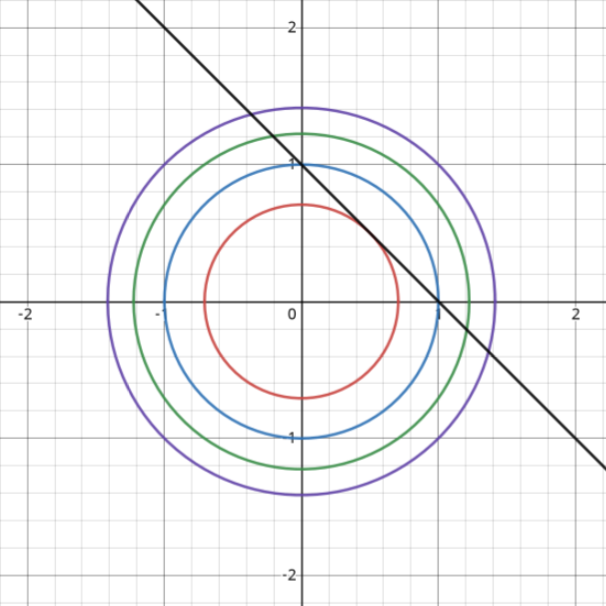
\includegraphics[width=0.5\textwidth]{figures/lagrange-visualization.png}
	\caption{Circles representing contour lines of the objective function intersect the black line defined by the constraint.}
\end{figure}

\begin{example}
	Let us see this with the help of the example discussed earlier.
	Contour lines of the function $f(x, y) = x^2 + y^2$ would be a series of circles, all centered at the origin $(0, 0)$, but of increasing radii.
	The curve $x + y = 1$ would be a line that cuts both the x and y axes at $+1$.
	The situation is illustrated in Figure \ref{lagrange-visualization}.
\end{example}

Then, the key point is this: the optimal solution of the problem \eqref{lagrange-constrained} must lie at the point where a contour line of $f(x)$ \textit{touches} the curve $g(x) = 0$.
Why?
First note that the optimal solution must lie at a point where a contour line of $f(x)$ intersects the curve $g(x) = 0$, or otherwise it would not satisfy the constraint in the first place.
And then, observe that it is not possible for this optimal solution to lie at a point where a contour line of $f(x)$ \textit{cuts across} the curve $g(x) = 0$, because then, along certain directions from this point of intersection, along the curve $g(x) = 0$, the value of the objective function $f(x)$ will increase and in certain other directions, its value will decrease.
At the point where a contour line of $f(x)$ touches the curve $g(x) = 0$, then, along all directions from this point of intersection, along the curve $g(x) = 0$, the value of the objective function $f(x)$ will only increase, indicating that this point is the minimum we are looking for.

\begin{example}
	Again, this will appear more convincing if we look at it in context of our example.
	Refer Figure \ref{lagrange-visualization}.
	Observe how the optimal solution cannot lie on any circle smaller than the red one, because such a circle would not intersect the black line at all and hence not satisfy the constraint.
	On the other hand, consider the points at which the black line intersects the blue, green and purple circles.
	Here, the circles cut across the line, and at each such point of intersection, observe that if we slide along the black line and go towards the origin, the value of $f(x, y)$ will decrease, and if we slide along the line and go away from the origin, the value of $f(x, y)$ will increase.
	However, if we look at the point at which the black line touches the red circle, we can try to slide along the black line and observe that in both directions along the line, the value of $f(x, y)$ will only increase.
	Hence, this point is the optimal solution of this problem.
\end{example}

Well, that makes sense, but what does this have to do with Lagrange multipliers and the problem \eqref{lagrange-unconstrained}?
The connection is as follows: from basic high school geometry, we know that the point at which two curves $f(x) = a$ and $g(x) = b$ touch, must satisfy one property -- that their slopes, i.e. their \textit{gradients}, at this point, must be parallel.
In other words,
\begin{equation*}
	\nabla f(x) = \lambda \nabla g(x)
\end{equation*}
This $\lambda$ is none other than our Lagrange multiplier!
Indeed, if you look at problem \eqref{lagrange-unconstrained}, and find its solution by taking the gradient of its objective function, $L(x, \lambda)$, with respect to $x$ and setting it to zero, then you will get a relation that is identical to the above.

\begin{example}
	Let us finally solve our example problem.
	We know that by the theory of Lagrange multipliers, it is equivalent to solving the problem
	\begin{equation*}
		\min \quad L(x, y, \lambda) = x^2 + y^2 - \lambda(x + y - 1)
	\end{equation*}
	Let us take the partial derivatives of $L$ with respect to $x$, $y$ and $\lambda$, and set them to zero since we want to find the optimal solution:
	\begin{align*}
		2x - \lambda & = 0 \\
		2y - \lambda & = 0 \\
		x + y - 1 & = 0
	\end{align*}
	Three equations, three variables.
	This system can be easily solved to yield the solution as:
	\begin{align*}
		x & = 0.5 \\
		y & = 0.5 \\
		\lambda & = 1
	\end{align*}
	Indeed, the point $(0.5, 0.5)$ is the point at which the black line touches the red circle in Figure \ref{lagrange-visualization}.
\end{example}

\subsection{Constrained Optimization}

The previous section on Lagrange multipliers dealt with a constrained optimization problem with a single equality constraint.
Now, let us look at the general form of a constrained optimization problem.
It goes as follows:
\begin{equation}
	\label{constrained-standard}
	\begin{aligned}
		\min \quad & f_0(x) \\
		\text{subject to} \quad & f_i(x) \leq 0, \quad \forall i = 1, 2, \dots, l \\
		& h_j(x) = 0, \quad \forall j = 1, 2, \dots, m
	\end{aligned}
\end{equation}
Essentially, we now allow multiple inequality constraints and multiple equality constraints.

The form \eqref{constrained-standard} is also called the \textit{standard form} of a constrained optimization problem, because every constrained optimization problem can be expressed in this form.
Let us see how:
\begin{itemize}
	\item A maximization problem
		\begin{equation*}
			\max \quad f_0(x)
		\end{equation*}
		can be converted into a minimization problem by taking the negation of the objective function:
		\begin{equation*}
			\min \quad -f_0(x)
		\end{equation*}
	\item An equality constraint with a nonzero right-hand side, such as
		\begin{equation*}
			x + y = 1
		\end{equation*}
		can be easily converted into a form with a zero on the right-hand side, i.e.
		\begin{equation*}
			x + y - 1 = 0
		\end{equation*}
		The same holds for an inequality constraint with a nonzero right-hand side.
	\item An inequality constraint involving $\geq$ instead of $\leq$, such as
		\begin{equation*}
			x + y \geq 1
		\end{equation*}
		can be easily handled as well, by taking the negation of both sides:
		\begin{equation*}
			- x - y \leq -1
		\end{equation*}
		(Negation of an inequality flips its sign.)
\end{itemize}
Basically, any constrained optimization problem, no matter what objective, equality constraints, or inequality constraints it has, can be converted into the form \eqref{constrained-standard}.

When we talk about constrained optimization problems, there are two important terms that we must keep in mind.
The first is the \textit{domain} -- the domain of the problem \eqref{constrained-standard} is the set of all $x$ for which all of the $l + 1$ functions $f_i$ and $m$ functions $h_j$ are defined.
On the other hand, the \textit{feasible set} of the problem \eqref{constrained-standard} is the set of all $x$ for which the constraints of the problem are satisfied.

The feasible set is always a subset of the domain.
For any $x$ to satisfy the constraints, it must lie in the domain of the problem first.

\begin{example}
	Let us consider a simple constrained optimization problem.
	This problem minimizes a linear objective, under what are known as \textit{box constraints}.
	\begin{align*}
		\min \quad & c^T x \\
		\text{subject to} \quad & l \preceq x \preceq u
	\end{align*}
	Here $x \in \mathbb{R}^n$ is the variable under optimization, while $c, l, u \in \mathbb{R}^n$ are the \textit{data} of the problem, i.e. the values given as part of the problem.

	The constraints are known as box constraints because the various elements of $x$ are restricted by boundaries on either side, and as such, the feasible set appears like a box.

	Let us look at the solution of this problem.
	The inequality constraint expressed using vectors can be expanded and written out as $n$ constraints of the form
	\begin{equation*}
		l_i \leq x_i \leq u_i
	\end{equation*}
	Now, the key observation is as follows.
	If $c_i \geq 0$ and we multiply it with each term in this inequality constraint, we have
	\begin{equation*}
		c_i l_i \leq c_i x_i \leq c_i u_i
	\end{equation*}
	On the other hand, if $c_i < 0$ and we multiply it with each term in this inequality constraint, we have
	\begin{equation*}
		c_i l_i \geq c_i x_i \geq c_i u_i
	\end{equation*}
	Note the reversal of signs in this case.

	Now the objective function can be written as
	\begin{equation*}
		c^T x = \sum_{i=1}^n c_i x_i
	\end{equation*}
	Focus on the individual terms $c_i x_i$.
	Realize that by the above inequalities, when $c_i \geq 0$, then the minimum value of the corresponding term $c_i x_i$ is $c_i l_i$, but when $c_i < 0$, then the minimum value of the corresponding term $c_i x_i$ is $c_i u_i$.

	Then, clearly, the optimal solution $x^* \in \mathbb{R}^n$ can be defined in terms of its elements as follows: for all $i$ from 1 to $n$, we have
	\begin{equation*}
		x_i^* =
		\begin{cases}
			l_i & \text{if } c_i \geq 0, \\
			u_i & \text{otherwise},
		\end{cases}
	\end{equation*}
	and we are done.
	But before we conclude, note a very neat result: that this expression tells us that the optimal solution will always lie at a corner of the box-shaped feasible set.
	We leave it to the reader to verify this.
\end{example}

\begin{example}
	Let us consider another simple constrained optimization problem.
	\begin{align*}
		\min \quad & c^T x \\
		\text{subject to} \quad & Ax \preceq b
	\end{align*}
	Here $x \in \mathbb{R}^n$ is the variable under optimization, while $c \in \mathbb{R}^n$, $A \in \mathbb{R}^{l \times n}$, and $b \in \mathbb{R}^l$ are the data of the problem.

	In this problem, we will assume that $l = n$, so $A$ is square, and additionally, we will also assume that $A$ has full rank, i.e. its rank is equal to $n$ as well.
	This essentially means that $A$ is invertible, and we intend to use this fact while solving this problem.

	The way we will find the solution of this problem is as follows.
	First, we set $y = Ax$.
	This implies that $x = A^{-1} y$.
	Then, our objective function, written in terms of $y$, becomes $c^T A^{-1} y$.
	Let us further write
	\begin{equation*}
		\tilde{c} = ( c^T A^{-1} )^T
	\end{equation*}
	so that our objective function becomes just $\tilde{c}^T y$.

	Then, let us rewrite our optimization problem in terms of $y$.
	\begin{align*}
		\min \quad & \tilde{c}^T y \\
		\text{subject to} \quad & y \preceq b
	\end{align*}
	You can see what has happened here.
	Essentially, the original variable of our optimization problem was $x \in \mathbb{R}^n$; we have replaced $x$ by a new variable $y \in \mathbb{R}^n$.

	You may have noticed the result of this transformation: our optimization problem suddenly becomes very straightforward to solve.
	Our constraint $y \preceq b$ can be written as $y_i \leq b_i$ for all $i = 1, \dots, n$.
	Our objective function is simply
	\begin{equation*}
		\sum_{i=1}^n \tilde{c}_i y_i
	\end{equation*}
	Then, on the lines of the previous example, if $\tilde{c}_i \geq 0$ for a certain $i$:
	\begin{equation*}
		\tilde{c}_i y_i \leq \tilde{c}_i b_i
	\end{equation*}
	but if $\tilde{c}_i < 0$ then
	\begin{equation*}
		\tilde{c}_i y_i \geq \tilde{c}_i b_i
	\end{equation*}

	Let us focus on the optimal value of the objective $\tilde{c}^T y$, and not on the optimal value of $y$.
	Realize that if $\tilde{c}_i < 0$ for a certain $i$, then the minimum value of the corresponding term $\tilde{c}_i y_i$ is $\tilde{c}_i b_i$, but if $\tilde{c}_i \geq 0$, then the minimum value of the corresponding term $\tilde{c}_i y_i$ is negative infinity!
	Now, if we look at the objective function, which is a sum of terms $\tilde{c}_i y_i$, observe that even if a single $\tilde{c}_i \geq 0$, then the negative infinity value of its corresponding term will bring down the entire sum to negative infinity.
	On the other hand, if all $\tilde{c}_i < 0$, each term in the summation will evaluate to $\tilde{c}_i b_i$, and then in this case the value of the objective function will be $\tilde{c}^T b$, or, substituting the value of $\tilde{c}$, it will be $c^T A^{-1} b$.

	Finally, we can write the solution of the problem as follows.
	At any optimal point $x^*$, the value of the objective function will be
	\begin{equation*}
		f_0(x^*) = \begin{cases}
			c^T A^{-1} b & \text{if } (A^T)^{-1} c \prec 0, \\
			-\infty & \text{otherwise.}
		\end{cases}
	\end{equation*}
	Here, we have used the component-wise inequality $(A^T)^{-1} c \prec 0$ to denote the case where all $\tilde{c}_i < 0$; note that $\tilde{c}$ is none other than $(A^T)^{-1} c$.
\end{example}

Now, let us discuss \textit{convex optimization} problems, which are a special and important category of constrained optimization problems.

Let us get right to the definition of a convex optimization problem.
A constrained optimization problem of the form \eqref{constrained-standard} is convex if and only if:
\begin{itemize}
	\item the objective $f_0$ is convex,
	\item the inequality constraint functions $f_i$ where $i = 1, \dots, l$ are all convex,
	\item and the equality constraint functions $h_j$ where $j = 1, \dots, m$ are all affine.
\end{itemize}

Why are convex optimization problems important?
One very useful property that they obey is as follows: any locally optimal point of a convex optimization problem, is also globally optimal.
The proof of this property is presented in Appendix \ref{proof-global-property}.

% TODO explain what is locally optimal and globally optimal, in the context of unconstrained optimization problems, and state that this will be more relevant when we talk about iterative algorithms for optimization.

Note that this property allows for multiple points to be globally optimal.
In other words, there can be multiple solutions that lead to the same globally optimal value of the objective.
This situation changes when the objective $f_0$ is strictly convex, instead of just being convex.
In that case, we are guaranteed to have only one, unique, global optimum.
The proof of this is simple and is left as an exercise to the reader.\footnote{
	Prove this by contradiction, using Jensen's inequality \eqref{jensen-inequality} for strictly convex functions, and take the help of Lemma \ref{feasible-convex}.
}
Intuitively, this can be understood as follows.
When the objective is a convex function that is not strictly convex, it is possible that a minimum found lies within a flat ``basin", surrounded by other equivalent minima.
However, when the objective is strictly convex, such flat ``basins" cannot exist, since the function is ``constantly" curving upwards.

\begin{example}
	\label{linear-program-example}
	Consider the optimization problem
	\begin{align*}
		\min \quad & c^T x \\
		\text{subject to} \quad & Cx \preceq d \\
		& Ax = b
	\end{align*}
	where $x \in \mathbb{R}^n$ is the variable under optimization, and $c \in \mathbb{R}^n$, $C \in \mathbb{R}^{l \times n}$, $d \in \mathbb{R}^l$, $A \in \mathbb{R}^{m \times n}$ and $b \in \mathbb{R}^m$ are the data of the problem.

	Is this problem convex?
	Let us see.
	The inequality constraint $Cx \preceq d$ can be written out as $l$ constraints of the form
	\begin{equation*}
		(i^\text{th} \text{ row of } C)^T x - d_i \leq 0
	\end{equation*}
	and similarly the equality constraint $Ax = b$ can be written out as $m$ constraints of the form
	\begin{equation*}
		(j^\text{th} \text{ row of } A)^T x - b_j = 0
	\end{equation*}
	Clearly the left-hand sides of both the inequality and equality constraints are all affine functions, the objective function is also affine, and affine functions are also convex.
	Hence, we have a convex objective function, convex inequality constraint functions, and affine equality constraint functions: the problem is convex.

	Such a problem, where all functions are affine, including the objective, the inequality constraint functions, and the equality constraint functions, is called a \textit{linear program (LP)}.
	These problems are an important subclass of convex optimization problems, and are often the simplest to solve.
\end{example}

\subsection{Duality and KKT Conditions}

In a previous section, we had discussed the theory of Lagrange multipliers, which presents a way to solve a constrained optimization problem with a single equality constraint.
The theory of duality and KKT conditions, discussed in this section, presents a way to solve constrained optimization problems in general.

Let us begin by rewriting \eqref{constrained-standard}, the standard form of a constrained optimization problem.
\begin{align*}
	\min \quad & f_0(x) \\
	\text{subject to} \quad & f_i(x) \leq 0, \quad \forall i = 1, 2, \dots, l, \\
	& h_j(x) = 0, \quad \forall j = 1, 2, \dots, m
\end{align*}
Note that at this point we make no assumption about the problem being convex, so the problem may be convex or non-convex.

When we discussed Lagrange multipliers, the main idea was to augment the objective function with a multiple (the Lagrange multiplier) of the constraint function.
The same idea is extended here, where we define a function known as the \textit{Lagrangian} to augment the objective function with a weighted sum of the constraint functions.
The Lagrangian associated with a problem of the form \eqref{constrained-standard} is defined as the function
\begin{equation}
	\label{lagrangian}
	L(x, \lambda, \nu) = f_0(x) + \sum_{i=1}^{l} \lambda_i f_i(x) + \sum_{j=1}^m \nu_j h_j(x)
\end{equation}
Note that $\lambda \in \mathbb{R}^l$ and $\nu \in \mathbb{R}^m$.

You can see how this is a generalization of the Lagrange multiplier idea.
In fact, the parameters $\lambda_i$ and $\nu_j$ are known as the Lagrange multipliers associated with their respective inequality and equality constraints.

Next, we define another function known as the \textit{Lagrange dual function}.
The Lagrange dual function associated with a problem of the form \eqref{constrained-standard} is defined as the minimum value of the Lagrangian, over all $x$ in the domain of the problem (denoted as $\mathcal{D}$), for a particular value of $\lambda$ and $\nu$.
\begin{equation}
	\label{lagrange-dual-function}
	g(\lambda, \nu) = \min_{x \in \mathcal{D}} L(x, \lambda, \nu)
\end{equation}

At this point we are ready to bring duality into the picture.
The first key point is this: associated with an optimization problem of the form \eqref{constrained-standard}, we define another optimization problem, known as the \textit{Lagrange dual problem} or simply as the \textit{dual problem}, as the problem that maximizes the Lagrange dual function over all nonnegative values of the $l$ Lagrange multipliers $\lambda_i$.
\begin{equation}
	\label{dual-problem}
	\begin{aligned}
		\max \quad & g(\lambda, \nu) \\
		\text{subject to} \quad & \lambda \succeq 0
	\end{aligned}
\end{equation}
In the context of this ``dual" problem, the original problem of the form \eqref{constrained-standard} is known as the \textit{primal problem}.

These dual and primal problems have a very interesting property. If $d^*$ is the optimal value of the dual problem, and $p^*$ is the optimal value of the primal problem, then we will always have
\begin{equation}
	\label{weak-duality}
	d^* \leq p^*
\end{equation}
This is the property of \textit{weak duality}.

Till now we have not assumed anything about whether the primal problem is convex or not.
Here comes the twist: typically, when the primal problem is convex, the inequality in \eqref{weak-duality} is replaced by equality:
\begin{equation}
	\label{strong-duality}
	d^* = p^*
\end{equation}
In other words, \textit{strong duality} holds.

Another property of the dual problem \eqref{dual-problem} is as follows: it is a convex optimization problem, whether the primal problem is convex or not.
This, along with weak and strong duality, are all very interesting properties that the dual problem has to offer.
Therefore, solving the dual problem often turns out to be very useful: solving the dual problem is either much easier than solving the primal problem, or the dual problem provides valuable insights about the primal problem.

More on how we arrive at the dual problem and the property of weak duality, along with a proof of the convexity of the dual problem, is discussed in Appendix \ref{derivation-duality}.

Why did we say that strong duality ``typically" holds if the primal problem is convex?
This is because, strictly speaking, convexity of the primal problem is not sufficient for strong duality to hold.
One condition under which strong duality holds given a convex primal problem is known as \textit{Slater's condition}.
This condition, loosely speaking, requires the feasible set to have an interior point.
We will not get too much into the details of this condition, or prove that strong duality holds when it is satisfied, because it requires a lot of rigorous math.
For our purposes, it is sufficient to remember that for many, many convex primal problems, Slater's condition is indeed satisfied, and strong duality does hold.

(There are several results that establish conditions on the primal problem, under which strong duality holds.
Such conditions are known as \textit{constraint qualifications}.
Slater's condition is one such constraint qualification.
Some constraint qualifications may not require the primal problem to be convex.)

With this background on duality, let us move on to the KKT conditions.
The \textit{Karush-Kuhn-Tucker (KKT)} conditions are an important set of conditions that characterize the optimal solutions of the primal and dual problems.
Without further ado, let us list these conditions ---

If $x^*$ is an optimal solution of the primal problem and $\lambda^*, \nu^*$ are an optimal solution of the dual problem, and strong duality holds, then the following conditions must hold:
\begin{enumerate}
	\item Primal constraints: the constraints of the primal problem must hold.
		\begin{align*}
			f_i(x^*) \leq 0, & \quad \forall i = 1, 2, \dots, l \\
			h_j(x^*) = 0, & \quad \forall j = 1, 2, \dots, m
		\end{align*}
	\item Dual constraints: the constraints of the dual problem must hold.
		\begin{equation*}
			\lambda^* \succeq 0
		\end{equation*}
	\item Complementary slackness: both the Lagrange multiplier and the inequality constraint cannot simultaneously be slack.
		\begin{equation*}
			\lambda_i^* f_i(x^*) = 0, \quad \forall i = 1, 2, \dots, l
		\end{equation*}
	\item Stationarity: the gradient of the Lagrangian with respect to $x$ must vanish. We must have
		\begin{align*}
			& \nabla_x L(x, \lambda^*, \nu^*) = 0 \\
			\Rightarrow \quad & \nabla f_0(x) + \sum_{i=1}^l \lambda_i^* \nabla f_i(x) + \sum_{j=1}^m \nu_j^* \nabla h_j(x) = 0
		\end{align*}
		at $x = x^*$.
\end{enumerate}
These are the KKT conditions.

The conditions numbered 1 and 2 should be self-explanatory, but numbers 3 and 4 require some explanation.
Let us start with condition number 3, named \textit{complementary slackness}.
First, note that the constraints of the primal and dual problems require $f_i(x) \leq 0$ and $\lambda_i \geq 0$ for all $i = 1, \dots, l$, respectively.
Now, the complementary slackness condition requires that the product of the Lagrange multiplier $\lambda_i$ and the corresponding inequality constraint function $f_i(x)$ be zero, for every $i$.
This essentially means that the Lagrange multiplier and the inequality constraint cannot both be \textit{slack}, i.e. have nonzero values, simultaneously:
\begin{itemize}
	\item If $\lambda_i > 0$, i.e. the Lagrange multiplier is slack, then its corresponding inequality constraint must be \textit{tight}, i.e. $f_i(x) = 0$.
	\item If $f_i(x) < 0$, i.e. the inequality constraint is slack, then its corresponding Lagrange multiplier must be tight, i.e. $\lambda_i = 0$.
\end{itemize}
Hence the name `complementary slackness'.

The reason for condition number 4, named \textit{stationarity} is very simple.
Consider the Lagrangian at the optimal values of $\lambda$ and $\nu$ as produced by the dual problem.
Then, it turns out that a minimizer of this Lagrangian, over all $x \in \mathcal{D}$, is none other than the optimal value of $x$ as produced by the primal problem.
Therefore, the gradient of the Lagrangian with respect to $x$ must be zero at this point.

Appendix \ref{kkt-derivation} contains derivations of how we arrive at the conditions numbered 3 and 4.

\begin{example}
	Let us consider a simple optimization problem:
	\begin{align*}
		\min \quad & \| x \|_2 \\
		\text{subject to} \quad & Ax = b
	\end{align*}
	Here, $x \in \mathbb{R}^n$ is the variable under optimization, and $A \in \mathbb{R}^{m \times n}$ and $b \in \mathbb{R}^m$ are the data of the problem.

	This problem requires us to minimize the Euclidean norm of a vector $x \in \mathbb{R}^n$, subject to some equality constraints.
	Such a problem is known as a \textit{least-norm} problem.
	Note that the problem is convex, because the norm is a convex function (Lemma \ref{norm-convex}), and the equality constraints are affine.

	Let us take a second look at the matrix equation $Ax = b$.
	From a linear algebra perspective, this is essentially a system of $m$ equations in $n$ variables.
	Realize that optimization makes sense only when we have an \textit{under-determined} system, i.e. we have more variables than we have equations and $m < n$.
	In this case, we will typically have more than one, and possibly infinite, number of solutions, and we can pose optimization as a problem through which we pick one of these solutions.
	In the case $m \geq n$, we will typically have either zero or one solution(s), and there is nothing to optimize over.

	Now, note that minimizing the Euclidean norm $\| x \|_2$ is equivalent to minimizing its square $\| x \|_2^2$, because the optimal value of $x$ will be the same in both cases.
	The square form is more convenient because it has a simple expression: it can be written as $x^T x$.
	Note also that the problem remains convex, because $x^T x$ is also a convex function in $x$.
	Then, our optimization problem becomes:
	\begin{align*}
		\min \quad & x^T x \\
		\text{subject to} \quad & Ax = b
	\end{align*}

	Let us now solve this problem using the KKT conditions.
	First, let us write the Lagrangian associated with this problem.
	Note the absence of the parameter $\lambda$, since there are no inequality constraints.
	\begin{align*}
		L(x, \nu) & = x^T x + \sum_{j=1}^m \nu_j \big( (j^\text{th} \text{ row of } A)^T x - b_j \big) \\
		& = x^T x + \nu^T (Ax - b)
	\end{align*}
	Let the optimal values of $x$ and $\nu$ be denoted by $x^*$ and $\nu^*$ respectively.
	Let us apply the stationarity condition, which states that the gradient of the Lagrangian with respect to $x$ must be zero at $x^*$.
	\begin{align*}
		& \nabla_x L(x, \nu^*) = 0 \\
		\Rightarrow \quad & 2x + A^T \nu^* = 0 \\
		\Rightarrow \quad & x^* = -\frac{1}{2} A^T \nu^*
	\end{align*}
	What is $\nu^*$?
	For this, we can use the KKT condition which states that the primal constraints must hold.
	This essentially translates to
	\begin{equation*}
		Ax^* = b
	\end{equation*}
	Now, we can substitute the expression for $x^*$ in terms of $\nu^*$ that we have just obtained:
	\begin{align*}
		& A \left( -\frac{1}{2} A^T \nu^* \right) = b \\
		\Rightarrow \quad & A A^T \nu^* = -2b \\
		\Rightarrow \quad & \nu^* = -2 (A A^T)^{-1} b
	\end{align*}
	Finally, we can back-substitute this value of $\nu^*$ into the expression for $x^*$, as follows:
	\begin{align*}
		x^* & = -\frac{1}{2} A^T \big( -2 (A A^T)^{-1} b \big) \\
		& = A^T (A A^T)^{-1} b
	\end{align*}
	This is the optimal solution!
\end{example}

\section{Applications}

\subsection{Support Vector Machines}

The \textit{support vector machine (SVM)} is a popular classification algorithm used in machine learning.
The SVM is a binary classifier, i.e. it separates points into two classes.
By default, it models a linear separation between the two classes, but it can be easily extended to model a non-linear separation as well.
In this section, we will discuss how we formulate the linear SVM as a convex optimization problem.

The training set for a binary classification problem essentially consists of a set of $M + N$ data points $x_i \in \mathbb{R}^n$, where (say) the first $M$ points belong to one class, and the remaining $N$ points belong to the other.
The goal, is to model a hyperplane -- a linear function of $x \in \mathbb{R}^n$ -- to separate the two classes.

Let us express this in concrete terms.
We want a hyperplane $a^T x + b = 0$, such that points belonging to one class lie on one side of the hyperplane, and points belonging to the other class lie on the other side.
This essentially means that we want to find parameters $a \in \mathbb{R}^n$ and $b \in \mathbb{R}$ such that
\begin{align*}
	a^T x_i + b > 0 \quad & \forall i = 1, 2, \dots, M, \\
	a^T x_i + b < 0 \quad & \forall i = M{+}1, M{+}2, \dots, M{+}N
\end{align*}

Now, this can be formulated as an optimization problem, where $a$ and $b$ are the variables we wish to optimize over, and the above inequalities are the constraints.
But, what do we want to optimize over?
At this point, there doesn't seem to be anything we would like to optimize over: after all, any hyperplane which satisfies the above inequalities is a valid classifier anyway.

Then, let us formulate this as an optimization problem with a trivial objective, i.e. we will minimize $C$ where $C$ is some constant.
\begin{align*}
	\min \quad & C \\
	\text{subject to} \quad & a^T x_i + b < 0 \quad \forall i = 1, 2, \dots, M, \\
	& a^T x_i + b > 0 \quad \forall i = M{+}1, M{+}2, \dots, M{+}N
\end{align*}
This problem may look odd, but it is meaningful.
Since the minimum of a constant is just the constant itself (for e.g. what is the minimum of 1?), this problem will simply ignore the objective function, and return any $a, b$ that satisfies the constraints.
Such a problem with a trivial objective function is also known as a \textit{feasibility problem}: an optimization problem that returns any feasible point.

We would like our problem to be convex.
The objective function, a constant, is trivially convex; the only issue is with the inequality constraints.
Observe that the inequality constraints are strict, i.e. they do not allow for equality, and if you recall the standard form \eqref{constrained-standard}, there is no way that we can have strict inequality constraints in a convex optimization problem.

Then, let us relax these strict inequality constraints to obtain the following problem:
\begin{align*}
	\min \quad & C \\
	\text{subject to} \quad & a^T x_i + b \leq 0 \quad \forall i = 1, 2, \dots, M, \\
	& a^T x_i + b \geq 0 \quad \forall i = M{+}1, M{+}2, \dots, M{+}N
\end{align*}
This problem seems alright, but it has an issue that is not so obvious.
That issue is this: realize that the trivial solution
\begin{equation*}
	a = 0, \quad b = 0
\end{equation*}
satisfies the constraints, and is feasible for this problem!
In other words, there is nothing stopping this problem from returning us this solution, which obviously makes no sense.
Realize that this was not the case before when the inequality constraints were strict.

Due to this issue, our optimization problem needs to be modified.
We modify the problem to use a \textit{slab} as the separation model: instead of a single hyperplane, we deal with two parallel hyperplanes.
These two hyperplanes can be governed by the equations
\begin{align*}
	a^T x + b & = 1 \\
	a^T x + b & = -1
\end{align*}
Note how the $a$ remains the same in both equations, since the hyperplanes must be parallel.

Then, the points belonging to one class will lie on one side of one of the hyperplanes, and the points belonging to the other class will lie on the other side of the other hyperplane.
With this, realize that the constraints become
\begin{align*}
	a^T x_i + b & \geq 1 && \forall i = 1, 2, \dots, M, \\
	a^T x_i + b & \leq -1 && \forall i = M{+}1, M{+}2, \dots, M{+}N
\end{align*}
Note how these constraints will not allow the trivial solution, so that issue is resolved.

Let us come back to the question of the objective function.
At this point, when we are using a slab as our separation model, we can choose a better objective function than the trivial one we chose earlier.
We can choose to find the ``thickest" slab, or, in other words, we can optimize to maximize the distance between the two parallel hyperplanes.
This will enable a more robust separation of the two classes, and reduce classification error.

A simple result states that given two parallel hyperplanes of the form $a^T x = b_1$ and $a^T x = b_2$, the (perpendicular) distance between them is given by the formula
\begin{equation*}
	\frac{| b_1 - b_2 |}{\| a \|_2}
\end{equation*}
Using this formula, we can find the distance between our two hyperplanes as well: it is
\begin{equation*}
	\frac{| (1 - b) - (-1 - b) |}{\| a \|_2} = \frac{2}{\| a \|_2}
\end{equation*}
Then this is the objective function we want to maximize!
Or, equivalently, we can simply minimize $\| a \|_2$!

Then, finally, the optimization problem takes the following form:
\begin{equation}
	\label{hard-linear-svm}
	\begin{aligned}
		\min \quad & \| a \|_2 \\
		\text{subject to} \quad & a^T x_i + b \geq 1 && \forall i = 1, 2, \dots, M, \\
		& a^T x_i + b \leq -1 && \forall i = M{+}1, M{+}2, \dots, M{+}N
	\end{aligned}
\end{equation}
This is the optimization problem that the linear SVM solves.
Note that $a \in \mathbb{R}^n$ and $b \in \mathbb{R}$ are the variables under optimization, and $x_i \in \mathbb{R}^n$ for all $i = 1, \dots, M{+}N$ are the data of the problem.

This optimization problem is clearly convex.
The objective function, a Euclidean norm, is convex (Lemma \ref{norm-convex}).
Additionally, the inequality constraint functions are affine in $a$ and $b$, and affine functions are also convex.
Hence the problem is convex.

Now, there is a catch.
In most practical problems, two classes are rarely perfectly separable in this manner.
There is always some spillover from one side to the other side, due to noise.
Hence, we have to modify our optimization problem to be able to tolerate some amount of unavoidable classification error.

How do we do this?
By introducing what are known as \textit{slack variables}.
For each data point $x_i$, we will introduce a slack variable $u_i$, which will tolerate some amount of classification error for this point.
These slack variables will be incorporated into our constraints as follows:
\begin{align*}
	a^T x_i + b & \geq 1 - u_i && \forall i = 1, 2, \dots, M, \\
	a^T x_i + b & \leq -1 + u_i && \forall i = M{+}1, M{+}2, \dots, M{+}N \\
	u_i & \geq 0 && \forall i = 1, 2, \dots, M{+}N
\end{align*}
You can see what is happening here.
Earlier, without these slack variables, we required data points $x_i$ to fall on one side of the slab or the other.
Now, these slack variables essentially loosen this requirement, by altering the right-hand sides of the inequalities so that some deviation from the numbers $1$ and $-1$ is allowed.
Also note how the slack variables are constrained to be nonnegative, because if they are not, then instead of loosening the separation between the two classes, they serve only to make it more strict.

We don't want too much slack, because that will result in too much classification error.
Hence we would like to minimize the total amount of slack.
For this, we will augment the previous objective function, which minimizes $\| a \|_2$, with a term corresponding to the total slack.
This total slack term can simply be a sum of the slack variables, i.e. $\sum_{i=1}^n s_i$, which is more concisely written in vector notation as $1^T u$, where ``$1$" really stands for an $M{+}N$-dimensional vector of ones.
The influence of the total slack term will be controlled by a parameter $\eta \geq 0$ that must be provided (i.e. it is not a variable to optimize over): a high $\eta$ means that we want very little slack, and a low $\eta$ means that we can tolerate some classification error.

So, our optimization problem now takes the following form:
\begin{equation}
	\label{soft-linear-svm}
	\begin{aligned}
		\min \quad & \| a \|_2 + \eta (1^T u) && \\
		\text{subject to} \quad & a^T x_i + b \geq 1 - u_i && \forall i = 1, 2, \dots, M, \\
		& a^T x_i + b \leq -1 + u_i && \forall i = M{+}1, M{+}2, \dots, M{+}N \\
		& u_i \geq 0 && \forall i = 1, 2, \dots, M{+}N
	\end{aligned}
\end{equation}
This formulation \eqref{soft-linear-svm} is known as the \textit{soft-margin} SVM, because it allows for ``soft" classification, while on the other hand the previous formulation \eqref{hard-linear-svm} is known as the \textit{hard-margin} SVM.
Here, $a \in \mathbb{R}^m$, $b \in \mathbb{R}$ and $u \in \mathbb{R}^{M{+}N}$ are the variables under optimization, and $x_i \in \mathbb{R}^n$ for all $i = 1, \dots, M{+}N$ along with the parameter $\eta$ are the data of the problem.
Note also that the problem still remains convex: the objective is convex in $a$ and affine in $u$, and the constraints are affine in $a$, $b$ and $u$.

\subsection{Diet Problem}

In this section, we will discuss an optimization problem known as the \textit{diet problem}.
The diet problem is a very simple linear program, whose dual problem has a rather interesting interpretation.

What is a linear program?
You may recall that we have seen this problem before in Example \ref{linear-program-example}.
A linear program (LP) is a convex optimization problem in which the objective function, the inequality constraint functions, and the equality constraint functions, are all affine.
\begin{equation}
	\label{linear-program}
	\begin{aligned}
		\min \quad & c^T x \\
		\text{subject to} \quad & Cx \preceq d \\
		& Ax = b
	\end{aligned}
\end{equation}

Let us find the dual of the general linear program \eqref{linear-program}.
First, let us write out the Lagrangian.
Note how we use vector notation, and also how we attempt to simplify its form by factoring $x$ out.
\begin{align*}
	L(x, \lambda, \nu) & = c^T x + \lambda^T (Cx - d) + \nu^T (Ax - b) \\
	& = x^T c + (x^T C^T - d^T) \lambda + (x^T A^T - b^T) \nu \\
	& = x^T (c + C^T \lambda + A^T \nu) - d^T \lambda - b^T \nu
\end{align*}
Then, the dual function is
\begin{equation*}
	g(\lambda, \nu) = \min_{x \in \mathbb{R}^n} L(x, \lambda, \nu)
\end{equation*}
Now, there is a key observation that we can make about the Lagrangian: it is affine in $x$.
This means that it really has no minimum with respect to $x$, i.e. it can go all the way down to $-\infty$!
Only under one scenario will this not happen: the scenario in which the coefficient of $x$ in its expression will be equal to zero, i.e. $c + C^T \lambda + A^T \nu = 0$.
In that case, its value will remain a constant $- d^T \lambda - b^T \nu$ for any value of $x$, and that will also be its minimum value.

This implies that
\begin{equation*}
	g(\lambda, \nu) = \begin{cases}
		- d^T \lambda - b^T \nu & \text{if } c + C^T \lambda + A^T \nu = 0, \\
		-\infty & \text{otherwise.}
	\end{cases}
\end{equation*}
Then, the dual problem simply maximizes this function over all $\nu$ and nonnegative $\lambda$.
But note that when this function is equal to $-\infty$, there is essentially nothing to maximize.
With that in mind, let us write out the dual problem as the following:
\begin{align*}
	\max \quad & - d^T \lambda - b^T \nu \\
	\text{subject to} \quad & \lambda \succeq 0 \\
	& c + C^T \lambda + A^T \nu = 0
\end{align*}
What we have done is that we have taken the condition under which the dual function assumes a non negative-infinity value, and inserted it as a constraint of our problem, so that we only attempt to maximize the non negative-infinity value.
This is the dual problem of the LP \eqref{linear-program}.
Notice that this dual problem is itself an LP, since the objective and constraint functions are all affine.

Strong duality holds.
The primal problem \eqref{linear-program} is convex, and Slater's condition holds as well.

At this point, we are ready to discuss the diet problem.
It goes as follows.
Suppose there are $m$ nutrients, such that $b_i$ is the minimum amount of nutrient $i$ that is required in a healthy diet.
There are also $n$ foods, and $c_j$ is the cost of purchasing one unit of food $j$.
Now, every food contains some amount of every nutrient.
Let $a_{ij}$ be the amount of nutrient $i$ contained within one unit of food $j$.

Then, the problem is to prepare a diet, where we must purchase some amount of each of the $n$ foods.
This diet must be healthy, i.e. for each of the $m$ nutrients, it must supply the mandatory minimum amount, and even more if possible.
However, this is counterbalanced by the need to minimize the total cost of purchasing the diet.
Given all of these things, the problem can be framed as:
\begin{align*}
	\min \quad & c^T x \\
	\text{subject to} \quad & Ax \succeq b \\
	& x \succeq 0
\end{align*}
Here, $x \in \mathbb{R}^n$ is a vector, whose each element $x_j$ denotes the amount in which we must purchase food $j$, and is the variable under optimization.
The data of the problem includes the vector $c \in \mathbb{R}^n$ which contains the costs $c_j$, the vector $b \in \mathbb{R}^m$ which contains the minimum nutritional amounts $b_i$, and the matrix $A \in \mathbb{R}^{m \times n}$ which contains the nutritional amounts per food $a_{ij}$.

Note how the objective and constraints of the problem have been framed; the last constraint requiring $x$ to be nonnegative is because we can't purchase food in negative amounts.
Clearly, this is an LP because its objective and constraint functions are all affine.

Let us evaluate the dual of this problem.
Following the steps we used to evaluate the dual of the LP \eqref{linear-program}, we first write out the Lagrangian.
\begin{align*}
	L(x, \lambda, \bar{\lambda}) & = c^T x + \lambda^T (- Ax + b) + \bar{\lambda}^T (-x) \\
	& = x^T (c - A^T \lambda - \bar{\lambda}) + b^T \lambda
\end{align*}
Note how we use two sets of Lagrange multipliers, $\lambda$ and $\bar{\lambda}$, to represent the two sets of inequality constraints.
Also note that we have to first reverse the signs of the inequality constraints, from $\succeq$ to $\preceq$, by taking the negation of both sides, so that they comply with the standard form \eqref{constrained-standard}.

Then, the dual problem is the following:
\begin{align*}
	\max \quad & b^T \lambda \\
	\text{subject to} \quad & \lambda \succeq 0 \\
	& \bar{\lambda} \succeq 0 \\
	& c - A^T \lambda - \bar{\lambda} = 0
\end{align*}
This is an optimization problem over two variables $\lambda$ and $\bar{\lambda}$.
Note how both are constrained to be nonnegative, because they are both Lagrange multipliers associated with inequality constraints.

However, there is one simplification we can make.
Note that $\bar{\lambda}$ does not figure in the objective function; it figures only in the last two constraints.
From the third constraint we have $\bar{\lambda} = c - A^T \lambda$, so the second constraint $\bar{\lambda} \succeq 0$ can be simply replaced by the constraint
\begin{align*}
	& c - A^T \lambda \succeq 0 \\
	\Rightarrow \quad & A^T \lambda \preceq c
\end{align*}
and we can get rid of the variable $\bar{\lambda}$.

Then, finally, the dual problem takes the form
\begin{align*}
	\max \quad & b^T \lambda \\
	\text{subject to} \quad & \lambda \succeq 0 \\
	& A^T \lambda \preceq c
\end{align*}
This is an optimization problem in only one variable, $\lambda$.

Let us see how we can interpret this dual problem.
Note that $\lambda \in \mathbb{R}^m$.
Then, suppose that each $\lambda_i$ denotes the price of synthetic pills that supply one unit of nutrient $i$.
We have a constraint $\lambda \succeq 0$, which ensures that prices cannot go in negative.

Then, look at the constraint $A^T \lambda \preceq c$.
These are basically $n$ inequalities of the form
\begin{equation*}
	\sum_{i=1}^m a_{ij} \lambda_i \leq c_j
\end{equation*}
Look at this inequality carefully.
The left-hand side is a summation of terms $a_{ij} \lambda_i$.
Realize that each such term denotes the price of pills of nutrient $i$, that will substitute the amount of this nutrient provided by food $j$!
And then, the summation of such terms denotes the total price of pills of all $m$ nutrients, that will substitute the entire nutritional value of this $j^\text{th}$ food.
Next, look at the right-hand side $c_j$, the cost of food $j$.
Then, you can see what these inequalities mean: the price of pills that can substitute the nutritional value of this food, must be lesser than or equal to the cost of the food itself.
And that is a natural requirement, because the synthetic pills will not sell unless they are cheaper (or not more expensive) than the food items from which we can get these same nutrients from!

Finally, look at the objective function.
Realize that $b^T \lambda$ is simply the total price of pills that will provide the minimum nutritional requirements of a healthy diet!
And we would like to maximize this price, so as to benefit the pill-seller.

Another point: strong duality holds, which leads to the following wonderful result.
The minimum cost at which a consumer buys a food-based healthy diet, is also the maximum price at which a pill-based healthy diet will sell!

The condition of complementary slackness also leads to some very interesting results.
In the optimal setting of both the food-based and pill-based diets, it turns out that:
\begin{itemize}
	\item If the food-based diet supplies more of nutrient $i$ than the minimum healthy requirement, then the pills of nutrient $i$ will sell for free.
		On the other hand, if the pills of nutrient $i$ have a nonzero price, than the food-based diet will supply only the minimum requirement of nutrient $i$.
	\item If the food-based diet includes nonzero quantities of food $j$, then the cost of food $j$ is the same as the price of its corresponding pills-based equivalent.
		On the other hand, if the pills-based equivalent sells at a lower price than the cost of food $j$, then the food-based diet does not include a purchase of food $j$.
\end{itemize}
We leave it as an exercise to the reader to see how these results come about.\footnote{
	Look at the Lagrange multipliers $\lambda$ and $\bar{\lambda}$ and their corresponding inequality constraints in the primal problem!
}
However, if you simply judge them intuitively, they do make a lot of sense.

The diet problem illustrates how there is a deep connection between the primal and dual problems, especially when strong duality holds.

\subsection{Logistic Regression}

\section{Algorithms}

\subsection{Newton-Raphson Method}

\subsection{Gradient Descent}

\section{References}

The material of this article has been primarily derived from two resources.
The first is the well-known book on Convex Optimization, by Stephen Boyd and Lieven Vandenberghe, published by Cambridge University Press, 2004.
The second is an online course titled ``Applied Optimization for Wireless, Machine Learning and Big Data," instructed by Prof. Aditya K. Jagannatham, of IIT Kanpur; his series of lectures can be found \href{https://youtube.com/playlist?list=PLFW6lRTa1g83Z2YAcz7kxrcPI2nJK6hjP}{here}.

Additionally, for some specific topics, the following resources have been consulted:
\begin{itemize}
	\item \href{https://youtu.be/GoyeNUaSW08}{Lecture} on Lagrange multipliers by Prof. S. K. Gupta of IIT Roorkee.
	\item \href{https://youtu.be/ZcbFQz_Kwog}{Lecture 1} and \href{https://youtu.be/b74LVxOazIQ}{lecture 2} on the Newton-Raphson method by Prof. R. Usha of IIT Madras.
	\item Chapter 8, titled ``Linear Programming and Game Theory", of the book ``Linear Algebra and its Applications", by Gilbert Strang, published by Cengage Learning, 2006.
\end{itemize}

\appendix

\section{Appendix}

\subsection{Convexity Results}
\label{convexity-results}

This section discusses certain simple results regarding the convexity of sets and functions.

\begin{lemma}
	\label{hyperplane-convex}
	A hyperplane is a convex set.
\end{lemma}
\begin{proof}
	Let $x, y \in \mathbb{R}^n$ lie on a hyperplane parameterized by some $a \in \mathbb{R}^n$ and $b \in \mathbb{R}$.
	Then
	\begin{equation*}
		a^T x + b = 0, \quad a^T y + b = 0
	\end{equation*}
	Then, for any $\theta$ such that $0 \leq \theta \leq 1$, we have
	\begin{align*}
		a^T (\theta x + (1 - \theta) y) + b & = \theta a^T x + (1 - \theta) a^T y + b \\
		& = \theta (a^T x + b) + (1 - \theta) (a^T y + b) \\
		& = \theta (0) + (1 - \theta) (0) \\
		& = 0
	\end{align*}
	which implies that $\theta x + (1 - \theta) y$ also lies on the hyperplane.
	Hence, the hyperplane is convex.
\end{proof}

The next result involves what is known as an $\alpha$\textit{-sublevel set}.
An $\alpha$-sublevel set of a function $f : \mathbb{R}^n \rightarrow \mathbb{R}$ is defined as the set of all $x \in \mathbb{R}^n$, such that $f(x) \leq \alpha$.
\begin{lemma}
	\label{sublevel-convex}
	For any value of $\alpha$, the $\alpha$-sublevel set of a convex function is convex.
\end{lemma}
\begin{proof}
	Let $x, y$ belong to the $\alpha$-sublevel set of a convex function $f$.
	Then
	\begin{equation*}
		f(x) \leq \alpha, \quad f(y) \leq \alpha
	\end{equation*}
	Taking into account the convexity of $f$, for any $\theta$ such that $0 \leq \theta \leq 1$, we have
	\begin{align*}
		f(\theta x + (1 - \theta)y) & \leq \theta f(x) + (1 - \theta) f(y) \\
		& \leq \theta \alpha + (1 - \theta) \alpha \\
		& = \alpha
	\end{align*}
	which implies that $\theta x + (1 - \theta) y$ also belongs to the $\alpha$-sublevel set.
	Hence, the $\alpha$-sublevel set is indeed convex.
\end{proof}

\begin{lemma}
	\label{convex-intersection}
	The intersection of two (or more) convex sets is convex.
\end{lemma}
\begin{proof}
	Let $A$ be a convex set and $B$ be another convex set.
	Consider two points $x, y \in A \cap B$.
	Then, by definition of the intersection of two sets, we have
	\begin{equation*}
		x, y \in A, \quad x, y \in B
	\end{equation*}
	Now, since $A$ is convex, and $x, y \in A$, for any $\theta$ such that $0 \leq \theta \leq 1$, we have
	\begin{equation*}
		\theta x + (1 - \theta) y \in A
	\end{equation*}
	and similarly for $B$:
	\begin{equation*}
		\theta x + (1 - \theta) y \in B
	\end{equation*}
	Then again, by definition of the intersection, $\theta x + (1 - \theta) y \in A \cap B$.
	Hence, the intersection of two convex sets is convex, and this can be easily generalized to the intersection of more than two convex sets as well.
\end{proof}

Now onto some results involving convex functions.
\begin{lemma}
	The negation of a concave function is convex.
\end{lemma}
\begin{proof}
	This is fairly straightforward.
	If the function $f$ is convex, then Jensen's inequality \eqref{jensen-inequality} must hold for $f$.
	If $g = -f$ is the negation of $f$, then it must satisfy Jensen's inequality with the sign reversed ($\leq$ replaced with $\geq$).
	This is the definition of a concave function.
	Hence $g$ must be concave.
\end{proof}

\begin{lemma}
	The sum of two (or more) convex functions is convex.
\end{lemma}
\begin{proof}
	This too is fairly straightforward.
	If two functions $f_1$ and $f_2$ are convex, then they must satisfy Jensen's inequality \eqref{jensen-inequality}.
	Let their sum be $f = f_1 + f_2$.
	Then, for all $x, y$ in the domain of $f_1$, $f_2$ as well as $f$, and for any $\theta$ such that $0 \leq \theta \leq 1$, we have
	\begin{align*}
		f(\theta x + (1 - \theta) y) & = f_1(\theta x + (1 - \theta) y) + f_2(\theta x + (1 - \theta) y) \\
		& \leq \big( \theta f_1(x) + (1 - \theta) f_1(y) \big) + \big( \theta f_2(x) + (1 - \theta) f_2(y) \big) \\
		& = \theta \big( f_1(x) + f_2(x) \big) + (1 - \theta) \big( f_1(y) + f_2(y) \big) \\
		& = \theta f(x) + (1 - \theta) f(y)
	\end{align*}
	This is Jensen's inequality for the function $f$; the inequality in the second step comes from Jensen's inequality for $f_1$ and $f_2$.
	Hence $f$, the sum of two convex functions, is convex.
\end{proof}

\begin{lemma}
	\label{norm-convex}
	The norm is a convex function.
\end{lemma}
\begin{proof}
	Using the properties of norms as discussed in Section \ref{norms}, for all $x, y \in \mathbb{R}^n$, and any $\theta$ such that $0 \leq \theta \leq 1$, we have
	\begin{align*}
		\| \theta x + (1 - \theta) y \| & \leq \| \theta x \| + \| (1 - \theta) y \| \\
		& = \theta \| x \| + (1 - \theta) \| y \|
	\end{align*}
	This is Jensen's inequality for the norm function.
	The first step is due to the triangle inequality, and the second is due to positive homogeneity.
	Hence the norm is convex.
\end{proof}

\begin{lemma}
	If $f : \mathbb{R}^m \rightarrow \mathbb{R}$ is a convex function, then the function $g : \mathbb{R}^n \rightarrow \mathbb{R}$ defined as
	\begin{equation*}
		g(x) = f(Ax + b)
	\end{equation*}
	where $A \in \mathbb{R}^{m \times n}$ and $b \in \mathbb{R}^m$, is also convex.
\end{lemma}
\begin{proof}
	If the function $f$ is convex, then Jensen's inequality \eqref{jensen-inequality} must hold for $f$.
	For all $x, y \in \mathbb{R}^n$, and any $\theta$ such that $0 \leq \theta \leq 1$, we have
	\begin{align*}
		g(\theta x + (1 - \theta) y) & = f \big( A (\theta x + (1 - \theta) y) + b \big) \\
		& = f ( \theta Ax + (1 - \theta) Ay + b) \\
		& = f \big( \theta (Ax + b) + (1 - \theta) (Ay + b) \big) \\
		& \leq \theta f(Ax + b) + (1 - \theta) f(Ay + b) \\
		& = \theta g(x) + (1 - \theta) g(y)
	\end{align*}
	This is Jensen's inequality for the function $g$.
	The third step is a result of some simple rearranging, noting that $b = \theta b + (1 - \theta) b$, and then in the fourth step, we use Jensen's inequality for the function $f$, noting that $Ax + b$ and $Ay + b$ both are points in $\mathbb{R}^m$, the domain of $f$.
	Hence the function $g$ is convex.
\end{proof}

The next result is a very important one.
It involves what is known as the \textit{epigraph} of a function: the set of points that lie on and above the graph of the function.
More explicitly, for a function $f : \mathbb{R}^n \rightarrow \mathbb{R}$, the epigraph of $f$ is defined as the set
\begin{equation*}
	\text{epi } f = \{ (x, y) \mid y \geq f(x) \}
\end{equation*}

\begin{lemma}
	\label{convex-epigraph}
	A function is convex if and only if its epigraph is convex.
\end{lemma}
\begin{proof}
	Let us first prove that a convex function has a convex epigraph.
	This proof is fairly straightforward.
	Let $(x_1, y_1) \in \text{epi } f$, and $(x_2, y_2) \in \text{epi } f$.
	Then, by definition of the epigraph,
	\begin{equation*}
		y_1 \geq f(x_1), \quad y_2 \geq f(x_2)
	\end{equation*}
	Since $f$ is convex, it satisfies Jensen's inequality, and for any $\theta$ such that $0 \leq \theta \leq 1$,
	\begin{align*}
		f(\theta x_1 + (1 - \theta) x_2) & \leq \theta f(x_1) + (1 - \theta) f(x_2) \\
		& \leq \theta y_1 + (1 - \theta) y_2
	\end{align*}
	Now, observe that by definition of the epigraph, this implies that
	\begin{equation*}
		\big( \theta x_1 + (1 - \theta) x_2, \; \theta y_1 + (1 - \theta) y_2 \big) \in \text{epi } f
	\end{equation*}
	Hence the epigraph is convex.

	Next, we need to prove that a function with a convex epigraph must be convex.
	Let us prove by contradiction and assume that $f$ is not convex.
	Then, there must exist points $x_1, x_2$ in its domain, as well as some $\theta$ such that $0 \leq \theta \leq 1$, which satisfy
	\begin{equation*}
		f(\theta x_1 + (1 - \theta) x_2) > \theta f(x_1) + (1 - \theta) f(x_2)
	\end{equation*}
	Now, note that corresponding to these two points $x_1$ and $x_2$, we have two points $(x_1, f(x_1))$ and $(x_2, f(x_2))$, which lie on the graph of $f$, and by definition of the epigraph, they also lie in the epigraph of $f$.
	Then, since the epigraph is convex, note that for any $\theta$ such that $0 \leq \theta \leq 1$, we have
	\begin{align*}
		\theta \big( x_1, f(x_1) \big) + (1 - \theta) \big( x_2, f(x_2) \big) & \in \text{epi } f \\
		\Rightarrow \big( \theta x_1 + (1 - \theta) x_2, \; \theta f(x_1) + (1 - \theta) f(x_2) \big) & \in \text{epi } f
	\end{align*}
	Now, observe that by definition of the epigraph, this implies that
	\begin{equation*}
		\theta f(x_1) + (1 - \theta) f(x_2) \geq f(\theta x_1 + (1 - \theta) x_2)
	\end{equation*}
	which is a contradiction of the inequality shown above.
	Hence, the function $f$ must be convex.
\end{proof}

\begin{lemma}
	The point-wise maximum of two (or more) convex functions is convex.
\end{lemma}
\begin{proof}
	Let $f$ and $g$ be two convex functions, and $h$ be their point-wise maximum, i.e. for any $x$ in the domain of both $f$ and $g$, we have
	\begin{equation*}
		h(x) = \max (f(x), g(x))
	\end{equation*}
	Now, let $(x_1, y_1)$ be any point in the epigraph of $h$. Then we will have
	\begin{equation*}
		y_1 \geq \max (f(x_1), g(x_1))
	\end{equation*}
	Realize that something that is greater than or equal to the maximum of two quantities, will be greater than or equal to each of those two quantities.
	Therefore
	\begin{equation*}
		y_1 \geq f(x_1), \quad y \geq g(x_1)
	\end{equation*}
	By definition of the epigraph, this means that the point $(x_1, y_1)$ lies in the epigraphs of both $f$ and $g$, or
	\begin{equation*}
		(x_1, y_1) \in \text{epi } f \cap \text{epi } g
	\end{equation*}
	Now, since $(x_1, y_1)$ is any point in the epigraph of $h$, this argument applies equally well to all points in the epigraph of $h$ and we can conclude that
	\begin{equation*}
		\text{epi } h \subseteq \text{epi } f \cap \text{epi } g
	\end{equation*}

	Next, we will prove the converse relationship, namely
	\begin{equation*}
		\text{epi } f \cap \text{epi } g \subseteq \text{epi } h
	\end{equation*}
	For this, let $(x_2, y_2)$ be any point that lies in the epigraphs of both $f$ and $g$, and then we have
	\begin{equation*}
		y_2 \geq f(x_2), \quad y_2 \geq g(x_2)
	\end{equation*}
	Then, on similar lines as the previous part, realize that something that is greater than or equal to two quantities, will be greater than or equal to the maximum of those two quantities, and
	\begin{align*}
		y_2 & \geq \max(f(x_2), g(x_2)) \\
		& = h(x_2)
	\end{align*}
	Hence, $(x_2, y_2)$ lies in the epigraph of $h$, and this applies equally well to all points in the intersection of the epigraphs of $f$ and $g$, which leads us to the relationship we were trying to prove.

	We now have two sets, namely $\text{epi } h$, and the intersection $\text{epi } f \cap \text{epi g}$, which are subsets of each other.
	Two sets being subsets of each other implies that both sets are, in fact, equal.
	In other words
	\begin{equation*}
		\text{epi } h = \text{epi } f \cap \text{epi } g
	\end{equation*}

	Now, by Lemma \ref{convex-epigraph}, the functions $f$ and $g$ are convex, so their epigraphs must be convex.
	By Lemma \ref{convex-intersection}, the intersection of two convex sets is a convex set.
	Therefore, the epigraph of $h$ is convex.
	Again, by Lemma \ref{convex-epigraph}, a function with a convex epigraph must be convex.
	Hence, $h$, the point-wise maximum of two convex functions, is a convex function.
\end{proof}

A corollary of this result is the following one:
\begin{lemma}
	\label{concave-point-wise-min}
	The point-wise minimum of two (or more) concave functions is concave.
\end{lemma}

\subsection{Proof of Global Optimality}
\label{proof-global-property}

In this section, we present the proof of the property that given a convex optimization problem, any locally optimal point is also globally optimal.

Let us turn to convex optimization problems of the form \eqref{constrained-standard}, and first look at an associated result:
\begin{lemma}
	\label{feasible-convex}
	The feasible set of a convex optimization problem is convex.
\end{lemma}
\begin{proof}
	The feasible set of a convex optimization problem of the form \eqref{constrained-standard} is an intersection of $l + m + 1$ sets.
	The first $l$ sets are of the form
	\begin{equation*}
		\{ x \in \mathbb{R}^n \mid f_i(x) \leq 0 \}
	\end{equation*}
	Note that each such set is a 0-sublevel set of a convex function $f_i$.
	Then, each of these $l$ sets are convex by Lemma \ref{sublevel-convex}.

	The following $m$ sets are of the form
	\begin{equation*}
		\{ x \in \mathbb{R}^n \mid h_j(x) = 0 \}
	\end{equation*}
	Here, the functions $h_j$ are affine, which means that they can expressed as a linear function of $x$, i.e. each of them are of the form $a^T x + b$ for a different $a \in \mathbb{R}^n$ and $b \in \mathbb{R}$.
	Then, each of these $m$ sets are hyperplanes and are convex by Lemma \ref{hyperplane-convex}.

	The last set is the domain $\mathcal{D}$ of the optimization problem, which itself is the intersection of $l + m + 1$ sets, comprising: the domain of the objective $f_0$, the domains of the $l$ inequality constraint functions $f_i$, and the domains of the $m$ equality constraint functions $h_j$.
	Now, the domains of the objective and the inequality constraint functions are convex sets, by definition of the corresponding functions being convex, and the domains of the equality constraint functions are none other than $\mathbb{R}^n$, by definition of them being affine, and $\mathbb{R}^n$ is a convex set.
	Clearly, the domain $\mathcal{D}$ is an intersection of convex sets, and then by Lemma \ref{convex-intersection}, this implies that the domain is a convex set.

	Returning to the feasible set, the same argument applies: it is an intersection of $l$ 0-sublevel sets, $m$ hyperplanes, and a domain, all of which are convex sets.
	Hence, the feasible set is convex.
\end{proof}

Note how this result implies that in a convex optimization problem, we are essentially minimizing a convex objective over a convex set.

Then, the proof of the property we wanted to prove goes as follows.
\begin{proof}
	A point $x^*$ is locally optimal for an optimization problem of the form \eqref{constrained-standard} if it minimizes $f_0$ in some vicinity of itself.
	Let us define this vicinity by a radius parameter $R > 0$.
	Then
	\begin{equation*}
		f_0(x^*) = \min \{ f_0(x) \mid x \text{ is feasible and } \| x - x^* \| \leq R \}
	\end{equation*}
	Let us prove by contradiction and assume that $x^*$ is not globally optimal.
	Then, there exists some $y$ such that $y$ is feasible and
	\begin{equation*}
		f_0(y) < f_0(x^*)
	\end{equation*}
	Note that by definition of $x^*$ being a local optimum, we must have
	\begin{equation*}
		\| y - x^* \| > R
	\end{equation*}
	Now consider the point $z$ given by
	\begin{equation*}
		z = \theta x^* + (1 - \theta) y
	\end{equation*}
	where we have
	\begin{equation*}
		\theta = 1 - \frac{R}{2 \| y - x^* \|}
	\end{equation*}
	Note how $0 \leq \theta \leq 1$.
	
	Then we have
	\begin{align*}
		\| z - x^* \| & = \| (1 - \theta) y - (1 - \theta) x^* \| \\
		& = (1 - \theta) \| y - x^* \| \\
		& = \frac{R}{2 \| y - x^* \|} \| y - x^* \| \\
		& = \frac{R}{2} \\
		& < R
	\end{align*}
	Next, note that by Lemma \ref{feasible-convex}, the feasible set of this problem is convex, and then, since $x^*, y$ are both feasible, and $0 \leq \theta \leq 1$, the point $z$ will also be feasible.

	Finally, note that since $f_0$ is convex, it will follow Jensen's inequality, and
	\begin{align*}
		f_0(z) & = f_0 (\theta x^* + (1 - \theta) y) \\
		& \leq \theta f_0 (x^*) + (1 - \theta) f_0(y) \\
		& < \theta f_0 (x^*) + (1 - \theta) f_0( x^* ) \\
		& = f_0 (x^*)
	\end{align*}
	In other words, we have a feasible point $z$ that lies in the vicinity of $x^*$ (as parameterized by the radius $R$), and minimizes $f_0$ more than $x^*$.
	This is a contradiction of $x^*$ being a local minimum.
	Hence, $x^*$ must be globally optimal.
\end{proof}

\subsection{Dual Problem and Weak Duality}
\label{derivation-duality}

In this section, we show how the dual problem and the property of weak duality can be derived.
We start with the Lagrange dual function \eqref{lagrange-dual-function}, which has some interesting properties.
The first one is as follows:
\begin{lemma}
	\label{dual-function-concave}
	The Lagrange dual function $g(\lambda, \nu)$ is concave in $\lambda$ and in $\nu$, even when the optimization problem it is associated with is not convex.
\end{lemma}
\begin{proof}
	If we fix a value of $x$ and plug it into the Lagrangian $L(x, \lambda, \nu)$ as shown in \eqref{lagrangian}, the Lagrangian becomes a linear function of both $\lambda$ and $\nu$, i.e. it is just a weighted sum of the various $\lambda_i$'s and $\nu_j$'s.
	In other words, upon fixing a value of $x$, the Lagrangian is affine in both $\lambda$ and $\nu$.
	Then, the Lagrange dual function, which minimizes the Lagrangian over all $x \in \mathcal{D}$, can be viewed as computing a point-wise minimum of a (possibly infinite) number of Lagrangians, each corresponding to a single unique value of $x$, and this is essentially a point-wise minimum of affine functions.
	Now, note that affine functions are also concave, since they do satisfy the opposite of Jensen's inequality \eqref{jensen-inequality} with equality.
	(In fact, affine functions are both concave and convex.)
	Then, by Lemma \ref{concave-point-wise-min}, we know that the point-wise minimum of concave functions is concave.
	Hence, the Lagrange dual function is concave, and this is irrespective of whether the associated optimization problem is convex or not.
\end{proof}

The next property of the Lagrange dual function that we shall discuss goes as follows.
Given any nonnegative $\lambda$, and any $\nu$, the Lagrange dual function is a lower bound to the optimal value of its associated optimization problem.

\begin{lemma}
	\label{dual-function-lower-bound}
	Denote the optimal value of the given optimization problem as $p^*$.
	Then, for any $\lambda \succeq 0$, and any $\nu$, we have
	\begin{equation*}
		g(\lambda, \nu) \leq p^*
	\end{equation*}
\end{lemma}
(Note the component-wise inequality notation, i.e. $\lambda \succeq 0$ implies $\lambda_i \geq 0$ for all $i = 1, \dots, l$.)

\begin{proof}
	Consider any point $\tilde{x}$ which is feasible in the given optimization problem.
	Additionally, take any $\lambda \succeq 0$ and any $\nu$.
	Now, evaluate the Lagrangian at this $\tilde{x}$, $\lambda$ and $\nu$:
	\begin{equation*}
		L(\tilde{x}, \lambda, \nu) = f_0(\tilde{x}) + \sum_{i=1}^l \lambda_i f_i(\tilde{x}) + \sum_{j=1}^m \nu_j h_j(\tilde{x})
	\end{equation*}
	Observe the terms of this Lagrangian.
	Realize that the term
	\begin{equation*}
		\sum_{j=1}^m \nu_j h_j(\tilde{x}) = 0
	\end{equation*}
	because each $h_j(\tilde{x}) = 0$, by definition of $\tilde{x}$ being feasible.
	Similarly, we have
	\begin{equation*}
		\sum_{i=1}^l \lambda_i f_i(\tilde{x}) \leq 0
	\end{equation*}
	because, each $f_i(\tilde{x}) \leq 0$ by definition of $\tilde{x}$ being feasible, and each $\lambda_i \geq 0$, so each product $\lambda_i f_i(\tilde{x})$ will be nonpositive, and the sum of such products will be nonpositive as well.

	Now, these two relations clearly imply that
	\begin{equation*}
		L(\tilde{x}, \lambda, \nu) \leq f_0(\tilde{x})
	\end{equation*}
	and then we can write
	\begin{align*}
		g(\lambda, \nu) & = \min_{x \in \mathcal{D}} L(x, \lambda, \nu) \\
		& \leq L(\tilde{x}, \lambda, \nu) \\
		& \leq f_0(\tilde{x})
	\end{align*}
	Let us explain this a little bit.
	In the first step, we write out the definition of the Lagrange dual function.
	The second step makes use of the following fact: the fact that the minimum over a set of quantities, must be lesser than or equal to any one of those quantities.
	In other words, the minimum of the Lagrangian over all $x \in \mathcal{D}$, must be lesser than or equal to the Lagrangian at a single chosen $x \in \mathcal{D}$, and that chosen $x$ can be $\tilde{x}$, a feasible point that must by definition lie in $\mathcal{D}$.
	Finally, the third step makes use of the inequality we have just discussed above.

	Carefully observe the result we have obtained.
	It implies that the Lagrange dual function is a lower bound, to the value of the objective function at any feasible point $\tilde{x}$.
	Now, consider a global minimum $x^*$, i.e. a point at which the value of the objective function is $p^*$.
	Since this global minimum is also just another feasible point, we can always put $\tilde{x} = x^*$ and the following relation will hold:
	\begin{align*}
		g(\lambda, \nu) & \leq f_0(x^*) \\
		& = p^*
	\end{align*}
	And this is precisely the inequality we wanted to prove.
\end{proof}

With this result, the question that arises is the following.
What is the best lower bound that we can get using the Lagrange dual function, for the optimal value $p^*$?
After all, a lower bound which is a very large negative number is of no good; we want a lower bound that is as close to $p^*$ as possible.
This can be framed as another optimization problem: the problem of maximizing the Lagrange dual function, while constraining $\lambda \succeq 0$.
Note how this problem is none other than our dual problem \eqref{dual-problem}!

The property of weak duality \eqref{weak-duality} naturally follows.
The dual problem \eqref{dual-problem} produces some optimal solution $(\lambda^*, \nu^*)$ that leads to a maximum value $d^*$ of the Lagrange dual function, which by Lemma \ref{dual-function-lower-bound} must be a lower bound to the optimal value $p^*$ of the primal problem, and we have weak duality \eqref{weak-duality}.

Before we conclude this section, here is a short proof of the fact that the dual problem is always a convex optimization problem, whether the primal problem is convex or not.
\begin{proof}
	We first need to write the dual problem \eqref{dual-problem} in standard form, i.e. as a problem of the form \eqref{constrained-standard}, where the objective is to minimize a function instead of maximizing it, and the inequality constraints use $\leq$ signs.
	\begin{align*}
		\min \quad & -g(\lambda, \nu) \\
		\text{subject to} \quad & -\lambda_i \leq 0, \quad \forall i = 1, 2, \dots, l
	\end{align*}
	This is an optimization problem with objective function $f_0(\lambda, \nu) = -g(\lambda, \nu)$, and inequality constraint functions $f_i(\lambda, \nu) = -\lambda_i$.
	There are no equality constraints.

	By Lemma \ref{dual-function-concave}, we know that the Lagrange dual function is concave, so its negation must be convex, and the objective function is convex.
	The inequality constraint functions are clearly affine, and affine functions are also convex, so the inequality constraint functions are convex.
	Hence, the problem is a convex optimization problem.
\end{proof}

\subsection{KKT Conditions}
\label{kkt-derivation}

In this section, we discuss the derivation of the KKT conditions.
Note that the conditions pertaining to the primal constraints and dual constraints are obvious, hence we will only derive the others pertaining to complementary slackness and stationarity.

Let $x^*$ be an optimal solution of the primal problem, and $\lambda^*, \nu^*$ be an optimal solution of the dual problem.
Assume strong duality \eqref{strong-duality} holds.
Then, we have
\begin{align*}
	f_0(x^*) & = g(\lambda^*, \nu^*) \\
	& = \min_{x \in \mathcal{D}} L(x, \lambda^*, \nu^*) \\
	& \leq L(x^*, \lambda^*, \nu^*) \\
	& = f_0(x^*) + \sum_{i=1}^l \lambda_i^* f_i(x^*) + \sum_{j=1}^m \nu_j^* h_j(x^*) \\
	& \leq f_0(x^*)
\end{align*}
Something very interesting is happening here: we have a chain of inequalities $f_0(x^*) \leq \dots \leq f_0(x^*)$.
Let us analyze the steps one by one.
The first step is a direct consequence of strong duality \eqref{strong-duality}: at the optimal points of the primal and dual problems, the values of their objective functions are the same.
In the second step, we essentially write out the definition of the Lagrange dual function, given $\lambda^*$ and $\nu^*$.
In the third step, we make use of the fact that the minimum of the Lagrangian over all $x \in \mathcal{D}$, is lesser than or equal to the Lagrangian at a single chosen $x \in \mathcal{D}$, namely the point $x^*$.
In the fourth step, we write out the full formula of the Lagrangian, given $x^*$, $\lambda^*$ and $\nu^*$.
Finally, in the fifth step, we make use of the fact that $x^*$ is a feasible point, and $\lambda^* \succeq 0$.

(For the third and fifth steps, recall the reasoning discussed in the proof of Lemma \ref{dual-function-lower-bound}.
A very similar reasoning has been used here as well.)

When we have such a chain of inequalities $f_0(x^*) \leq \dots \leq f_0(x^*)$, this implies that all intermediate quantities in this chain must be equal to $f_0(x^*)$ and to each other.
(If this doesn't sound convincing, consider this example chain: $5 \leq x \leq y \leq 5$.
What will be the values of $x$ and $y$?)

Let us consider an equality relation derived from steps two and three of this chain:
\begin{equation*}
	\min_{x \in \mathcal{D}} L(x, \lambda^*, \nu^*) = L(x^*, \lambda^*, \nu^*)
\end{equation*}
What this relation implies is that given $\lambda^*$ and $\nu^*$, the point $x^*$ is a minimizer of the Lagrangian over all $x \in \mathcal{D}$.
Then, the Lagrangian must have a zero gradient with respect to $x$ at the point $x^*$, and this completes the derivation of the stationarity condition.

We are left with the complementary slackness condition.
For this, consider the equality relation derived from steps four and five of this chain:
\begin{equation*}
	f_0(x^*) + \sum_{i=1}^l \lambda_i^* f_i(x^*) + \sum_{j=1}^m \nu_j^* h_j(x^*) = f_0(x^*)
\end{equation*}
Realize that since $x^*$ is a feasible point, each $h_j(x^*) = 0$, and then, what is left of this relation is the following:
\begin{equation*}
	\sum_{i=1}^l \lambda_i^* f_i(x^*) = 0
\end{equation*}
Noting that $x^*$ is a feasible point and $\lambda^* \succeq 0$, each term $\lambda_i^* f_i(x^*)$ will be nonpositive.
(Again, recall the reasoning discussed in the proof of Lemma \ref{dual-function-lower-bound}.)
Now, observe that a sum of nonpositive quantities will be equal to zero, only when each of these nonpositive quantities is equal to zero.
Hence, we can conclude that
\begin{equation*}
	\lambda_i^* f_i(x^*) = 0 \quad \forall i = 1, 2, \dots, l
\end{equation*}
This is the complementary slackness condition, and that completes our derivation.

\end{document}
